\documentclass[12pt,a4paper]{article}
\usepackage[utf8]{inputenc}
%\usepackage[T1]{fontenc}
\setlength{\parindent}{0cm}
\setlength{\parskip}{\baselineskip}
\usepackage{amsmath}
\usepackage{amsfonts}
\usepackage{amssymb}
\usepackage{graphicx}
\author{Jean-François Mercier}
\title{Market Wage of Restricted Professional Baseball Players \\ Overview of the Methodology}

\begin{document}
\maketitle

\section{Summary}

From a labor market perspective, professional baseball players in the Major League Baseball (MLB) fall into two categories\footnote{Unofficial terms used for simplicity. The reality is more complex. There are more than two classes.}: restricted and unrestricted agents. Restricted agents are players whose rights to play are owned by the team that hires them. If a restricted player's contract comes to an end, unless granted free agency, a restricted player is limited in his work supply. Namely, a restricted player can either only supply work for one team or, may supply work for other teams while granting the team that owns the player's right  some compensation or comparative advantage over the player's work supply. Economic theory would suggests that a restricted player gets paid a wage that is at most equal to its market wage and most probably below it. Market frictions may block other teams from making offers or may induce additional costs to prospective teams who would otherwise make an offer to the player. 

Unrestricted agents, commonly known as free agents, can supply work to any team of their choosing, once their current contract has expired. We believe that free agents get paid their fair market wage. Without market frictions, free agents shall get paid what the market offers given all publicly available information.  

\subsection{Research question}
\begin{enumerate}
	\item For any given unrestricted agent, what is the best estimate of its market wage using only batting, fielding and pitching data?
	\item What are the economic factors that can explain the difference between market wage and observed wage for restricted player?
\end{enumerate}

\section{Methodology}

\subsection{Data}

Data comes from baseball-reference.com. We have batting, fielding and pitching data for every player and every game each player took part in, for all seasons from 2000 to 2019. We also have data on individual characteristics such as date of birth, nationality, height, weight, draft rank and more. Finally, we have salary data that come from  baseball-reference.com and other sources, namely baseball-almanac.com and spotrac.com. For every player in our sample, we have an indicator that tells whether or not a player was restricted during the current season. That way, we can separate restrict from unrestricted. 

Here is an small sample of our data set:

\begin{figure}[!h]
	\centering
	\caption[Example of our Data]{}
	\label{fig:dataex1}
	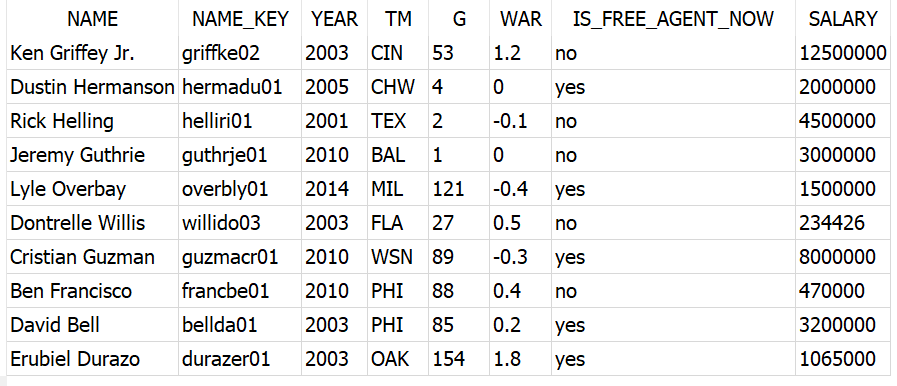
\includegraphics[width=1\linewidth]{data_ex1}
\end{figure}

\subsection{Predicting market wage}

In order to predict market wage, we need to separate restricted from unrestricted agents. Then, use only the unrestricted agents, \textit{i.e} those for whom "IS\_FREE\_AGENT\_NOW" = "yes", and train a Machine Learning model and subsequently apply it on the restricted agents.

Let $X_{U}$ be the matrix of features of unrestricted agents and $y_{U}$ a vector of salaries for the unrestricted agents. $X_{U}$ is of size $m\times n$, and $y_U$ is of size $m\times 1$. Similarly, I will use the subscript $R$ to denote the restricted agents. Let $f$ be the ML model that performs best at predicting $y_{U}$ from $X_{U}$. $f$ could be a linear regression, a regression tree, a neural network, or any other model that performs best. At this point, the objective is to be as precise as possible in predicting $y_U$.

Once we have chosen $f$, the parameters $\theta$ have been fitted according to  $X_{U}$ and $y_{U}$.  So for instance, salaries predicted by $f$ from $X_U$ given $\theta$ are \[\hat{y}_U = f(X_U|\ \theta),\] and $f$ and $\theta$ could satisfy, 
\[\min_{f,\theta} \sum_{i=1}^{m} \left( y_U^{(i)} - \hat{y}_U^{(i)}\right)^2,\] if minimizing the sum of squared errors is the metric we decide to use.


\subsection{Explaining the gap between observed wage and predicted market wage}

The vector of predicted market wages for the restricted free agents is
\[\hat{y}_R = f(X_R|\ \theta),\] and what I want to explain is the vector
\[\hat{y}_R - y_R.\]

I view this as an econometric problem and I believe that linear models are more appropriate for this task. 
I do not exactly have a good idea on what is the best procedure, though. What should I regress $\hat{y}_R - y_R$ on? Should we make sure that the variables in this regression do not overlap with the variables used in the first part? What is the possible issue in using the same variables in two regressions? 

At first glance, I would regress $\hat{y}_R - y_R$ on variables that do not overlap with the variables used in the first part so that we can isolate baseball related data (batting, fielding and pitching) in the first step and only focus on economic variables in the second step. Variables such has average income per capita, population size of home team city, team fixed effect, history of championships and so on.

I would love to have your suggestions on this matter.
\end{document}